\documentclass[letterpaper]{book}
\usepackage[utf8]{inputenc}
\usepackage[spanish]{babel}
\usepackage{amsmath}
\usepackage{amssymb}
\usepackage{graphicx}
\usepackage{multirow}
\usepackage{hyperref}
\usepackage{listings}
\usepackage{color}
\usepackage{schemata}
\usepackage{float}
\usepackage[left=2.00cm, right=1.00cm, top=2.00cm, bottom=2.00cm]{geometry}
\decimalpoint

\newcommand{\req}{$ \boxtimes $}
\newcommand{\nreq}{$ \Box $}

\definecolor{keywordColor}{RGB}{0, 0, 230}
\definecolor{stringColor}{RGB}{206, 123, 0}
\definecolor{commentColor}{RGB}{150, 150, 150}
\lstset{breaklines=true, keywordstyle=\color{keywordColor}, stringstyle=\color{stringColor}, commentstyle=\color{commentColor}, basicstyle=\footnotesize, extendedchars=true, inputencoding=utf8}

\newcommand{\cuadrosinoptico}[2]{\schema{\schemabox{#1}}{\schemabox{#2}}}

\begin{document}

\author{Rubén Ramírez}
\title{Zend Django App}
% \date{January 2013}

\frontmatter
\maketitle
\tableofcontents
\listoffigures

\mainmatter
\chapter{Modelos y Autenticación}

\section{django.contrib.auth.backends}

\begin{itemize}
	\item BaseBackend
	\item ModelBackend
	\item AllowAllUsersModelBackend
	\item RemoteUserBackend
	\item AllowAllUsersRemoteUserBackend
\end{itemize}

\section{django.contrib.auth.models}

\begin{itemize}
	\item User
	\item UserManager
	\item AnonymousUser
	\item Permission
	\item Group
\end{itemize}

\section{django.contrib.auth.validators}

\begin{itemize}
	\item ASCIIUsernameValidator
	\item UnicodeUsernameValidator
\end{itemize}

\chapter{Base de Datos}

\section{auth\_group}

\begin{tabular}{|l|l|l|l|l|l|}
	\hline
	\textbf{Campo} & \textbf{Tipo} & \textbf{Pk} & \textbf{NN} & \textbf{U} & \textbf{Referencia} \\
	\hline
	id & integer & \req & \req & \req & \\
	name & varchar(150) & \nreq & \req & \req & \\
	\hline
\end{tabular}

\section{auth\_group\_permissions}

\begin{tabular}{|l|l|l|l|l|l|}
	\hline
	\textbf{Campo} & \textbf{Tipo} & \textbf{Pk} & \textbf{NN} & \textbf{U} & \textbf{Referencia} \\
	\hline
	id & integer & \req & \req & \req & \\
	group\_id & integer & \nreq & \req & \nreq & auth\_group.id \\
	permission\_id & integer & \nreq & \req & \nreq & auth\_permission.id \\
	\hline
\end{tabular} \\ 

Grupos únicos:

\begin{itemize}
	\item (group\_id, permission\_id)
\end{itemize}

\section{auth\_permission}

\begin{tabular}{|l|l|l|l|l|l|}
	\hline
	\textbf{Campo} & \textbf{Tipo} & \textbf{Pk} & \textbf{NN} & \textbf{U} & \textbf{Referencia} \\
	\hline
	id & integer & \req & \req & \req & \\
	content\_type\_id & integer & \nreq & \req & \nreq & django\_content\_type.id \\
	codename & varchar(100) & \nreq & \req & \nreq & \\
	name & varchar(255) & \nreq & \req & \nreq & \\
	\hline
\end{tabular} \\ 

Grupos únicos:

\begin{itemize}
	\item (content\_type\_id, codename)
\end{itemize}

\section{auth\_user}

\begin{tabular}{|l|l|l|l|l|l|}
	\hline
	\textbf{Campo} & \textbf{Tipo} & \textbf{Pk} & \textbf{NN} & \textbf{U} & \textbf{Referencia} \\
	\hline
	id & integer & \req & \req & \req & \\
	password & varchar(128) & \nreq & \req & \nreq & \\
	last\_login & datetime & \nreq & \nreq & \nreq & \\
	is\_superuser & bool  & \nreq & \req & \nreq & \\
	username & varchar(150) & \nreq & \req & \req & \\
	first\_name & varchar(30) & \nreq & \req & \nreq & \\
	email & varchar(254) & \nreq & \req & \nreq & \\
	is\_staff & bool & \nreq & \req & \nreq & \\
	is\_active & bool & \nreq & \req & \nreq & \\
	date\_joined & datetime & \nreq & \req & \nreq & \\
	last\_name & varchar(150) & \nreq & \req & \nreq & \\
	\hline
\end{tabular}

\section{auth\_user\_groups}

\begin{tabular}{|l|l|l|l|l|l|}
	\hline
	\textbf{Campo} & \textbf{Tipo} & \textbf{Pk} & \textbf{NN} & \textbf{U} & \textbf{Referencia} \\
	\hline
	id & integer & \req & \req & \req & \\
	user\_id & integer & \nreq & \req & \nreq & auth\_user.id \\
	group\_id & integer & \nreq & \req & \nreq & auth\_group.id \\
	\hline
\end{tabular} \\ 

Grupos únicos:

\begin{itemize}
	\item (user\_id, group\_id)
\end{itemize}

\section{auth\_user\_user\_permissions}

\begin{tabular}{|l|l|l|l|l|l|}
	\hline
	\textbf{Campo} & \textbf{Tipo} & \textbf{Pk} & \textbf{NN} & \textbf{U} & \textbf{Referencia} \\
	\hline
	id & integer & \req & \req & \req & \\
	user\_id & integer & \nreq & \req & \nreq & auth\_user.id \\
	permission\_id & integer & \nreq & \req & \nreq & auth\_permission.id \\
	\hline
\end{tabular} \\

Grupos únicos:

\begin{itemize}
	\item (user\_id, permission\_id)
\end{itemize}

\section{django\_admin\_log}

\begin{tabular}{|l|l|l|l|l|l|}
	\hline
	\textbf{Campo} & \textbf{Tipo} & \textbf{Pk} & \textbf{NN} & \textbf{U} & \textbf{Referencia} \\
	\hline
	id & integer & \req & \req & \req & \\
	action\_time & datetime & \nreq & \req & \nreq & \\
	object\_id & text & \nreq & \nreq & \nreq & \\
	object\_repr & varchar(200) & \nreq & \req & \nreq & \\
	change\_message & text & \nreq & \req & \nreq & \\
	content\_type\_id & integer & \nreq & \nreq & \nreq & django\_content\_type.id \\
	user\_id & integer & \nreq & \req & \nreq & auth\_user.id \\
	action\_flag & smallint unsigned & \nreq & \req & \nreq & \\
	\hline
\end{tabular}

\section{django\_content\_type}

\begin{tabular}{|l|l|l|l|l|l|}
	\hline
	\textbf{Campo} & \textbf{Tipo} & \textbf{Pk} & \textbf{NN} & \textbf{U} & \textbf{Referencia} \\
	\hline
	id & integer & \req & \req & \req & \\
	app\_label & varchar(100) & \nreq & \req & \nreq & \\
	model & varchar(100) & \nreq & \req & \nreq & \\
	\hline
\end{tabular} \\

Grupos únicos:

\begin{itemize}
	\item (app\_label, model)
\end{itemize}

\section{django\_migrations}

\begin{tabular}{|l|l|l|l|l|l|}
	\hline
	\textbf{Campo} & \textbf{Tipo} & \textbf{Pk} & \textbf{NN} & \textbf{U} & \textbf{Referencia} \\
	\hline
	id & integer & \req & \req & \req & \\
	app & varchar(255) & \nreq & \req & \nreq & \\
	name & varchar(255) & \nreq & \req & \nreq & \\
	applied & datetime & \nreq & \req & \nreq & \\
	\hline
\end{tabular}

\section{django\_session}

\begin{tabular}{|l|l|l|l|l|l|}
	\hline
	\textbf{Campo} & \textbf{Tipo} & \textbf{Pk} & \textbf{NN} & \textbf{U} & \textbf{Referencia} \\
	\hline
	session\_key & varchar(40) & \req & \req & \req & \\
	session\_data & text & \nreq & \req & \nreq & \\
	expire\_date & datetime & \nreq & \req & \nreq & \\
	\hline
\end{tabular}
\chapter{Diagrama de Clases}

\section{django.contrib.auth.models}

\begin{tabular}{|l|}
	\hline
	\textbf{User} \\
	\hline
	username: string(150) \\
	first\_name: string(30) \\
	last\_name: string(30) \\
	email: email \\
	password: hash \\
	groups: Group[ ] \\
	user\_permissions: Permission[ ] \\
	is\_staff: boolean \\
	is\_active: boolean \\
	is\_superuser: boolean \\
	last\_login: datetime \\
	date\_joined: datetime \\
	\hline
	is\_authenticated: boolean \\
	is\_anonymous: boolean \\
	\hline
	get\_username(): string \\
	get\_full\_name(): string \\
	get\_short\_name(): string \\
	set\_password(raw\_password) \\
	check\_password(raw\_password): boolean \\
	set\_unusable\_password() \\
	has\_usable\_password(): boolean \\
	get\_user\_permissions(obj=None): string[ ] \\
	get\_group\_permissions(obj=None): string[ ] \\
	get\_all\_permissions(obj=None): string[ ] \\
	has\_perm(perm, obj=None): boolean \\
	has\_perms(perm[ ], obj=None): boolean \\
	has\_module\_perms(app\_label): boolean \\
	email\_user(subject, message, from\_email=None, **kwargs) \\
	\hline
\end{tabular}\\

\begin{tabular}{|l|}
	\hline
	\textbf{UserManager: BaseUserManager} \\
	\hline
	\\
	\hline
	create\_user(username, email=None, password=None, **extra\_fields): User \\
	create\_superuser(username, email=None, password=None, **extra\_fields) \\
	with\_perm(perm, is\_active=True, include\_superusers=True, backend=None, obj=None): User[ ] \\
	\hline
\end{tabular}\\

\begin{tabular}{|l|}
	\hline
	\textbf{Permission} \\
	\hline
	name: string \\
	content\_type: +django\_content\_type \\
	codename: string \\
	\hline
	\\
	\hline
\end{tabular}\\

\begin{tabular}{|l|}
	\hline
	\textbf{Group} \\
	\hline
	name: string \\
	permissions:  Permission[ ] \\
	\hline
	\\
	\hline
\end{tabular}\\

Formatos:

\begin{itemize}
	\item perm: ``app\_label.permission\_codename"
\end{itemize}

\section{django.contrib.contenttypes.models}

\begin{tabular}{|l|}
	\hline
	\textbf{ContentType} \\
	\hline
	app\_label: string \\
	model: string \\
	name: string \\
	\hline
	get\_object\_for\_this\_type(**kwargs): \textit{ModelClassObjects} \\
	model\_class(): \textit{ModelClass} \\
	\hline
\end{tabular}\\

\begin{tabular}{|l|}
	\hline
	\textbf{ContentTypeManager} \\
	\hline
	\\
	\hline
	clear\_cache() \\
	get\_for\_id(id): ContentType \\
	get\_for\_model(model, for\_concrete\_model=True): ContentType \\
	get\_for\_models(*models, for\_concrete\_model=True): dict \\
	get\_by\_natural\_key(app\_label, model): ContentType \\
	\hline
\end{tabular}\\

\section{django.contrib.auth.base\_user}

\begin{tabular}{|l|}
	\hline
	\textbf{AbstractBaseUser} \\
	\hline
\end{tabular}

\begin{tabular}{|l|}
	\hline
	\textbf{UserManager} \\
	\hline
\end{tabular}

\section{Otros}

\begin{tabular}{|l|}
	\hline
	\textbf{BaseUserManager} \\
	\hline
	\\
	\hline
	\textit{static} normalize\_email(email): string \\
	get\_by\_natural\_key(username): User \\
	make\_random\_password(length=10, allowed\_chars= \\ 
	\hphantom{spaces} 'abcdefghjkmnpqrstuvwxyzABCDEFGHJKLMNPQRSTUVWXYZ23456789'): string \\
	\hline
\end{tabular}

\section{zend\_django.functional\_tests.utils\_test}

\begin{tabular}{|l|}
	\hline
	\textbf{FuncionalTest: StaticLiveServerTestCase} \\
	\hline
	main\_model\_name: string = ``'' \\
	base\_data\_model: model = None \\
	duplicar: string = ``alfa'' \\
	actualizar1: string = ``beta'' \\
	actualizar2: string = ``beta\_002'' \\
	\hline
	setUp() \\
	tearDown() \\
	xPathFind(xpath, multiple=False, base\_object = None) \\
	Wait2PresenceOf(xpath, seconds=30) \\
	t\_list(search\_text=``alfa'') \\
	t\_list\_to\_crud\_pages() \\
	t\_read\_to\_crud\_pages() \\
	t\_update\_right() \\
	\hline
\end{tabular} \\

\begin{tabular}{|l|}
	\hline
	\textbf{URLsTests: SimpleTestCase} \\
	\hline 
	model\_name: string = ``'' \\
	main\_views: views\_modelule = None \\
	\hline
	t\_url\_resolves(url, view) \\
	t\_list\_url\_resolves() \\
	t\_crerate\_url\_resolves() \\
	t\_update\_url\_resolves() \\
	t\_delete\_url\_resolves() \\
	t\_read\_url\_resolves() \\
	\hline
\end{tabular} \\

\begin{tabular}{|l|}
	\hline
	\textbf{ViewsTests: TestCase} \\
	\hline
	model\_name: string = ``'' \\
	duplicar: string = ``alfa'' \\
	actualizar1: string = ``beta'' \\
	actualizar2: string = ``beta\_002'' \\
	inexistente: string = ``inexistente'' \\
	idinexistente: int = 99999 \\
	main\_views: views\_module = None \\
	campo\_base: string = ``'' \\
	base\_data\_model: model = None \\
	objs: data\_object = [] \\
	\hline
	getData(obj) \\
	preSetUp() \\
	t\_list\_get\_post(method=``get'') \\
	t\_list\_post\_searching() \\
	t\_list\_post\_no\_searching() \\
	t\_list\_post\_searching\_inexistent() \\
	t\_list\_post\_no\_searching\_inexistent() \\
	t\_read\_get\_existente(template\_file=``zend\_django/html/form.html'') \\
	t\_read\_get\_inexistente() \\
	t\_read\_post(id) \\
	t\_create\_get\_post(looking\_for, method=``get'', template\_file=``zend\_django/html/form.html'') \\
	t\_create\_post\_well(data=None) \\
	t\_create\_post\_duplicating(looking\_for, data=None, template\_file=``zend\_django/html/form.html'') \\
	t\_update\_get\_post(id, looking\_for, method=``get'', template\_file=``zend\_django/html/form.html'') \\
	t\_update\_get\_inexistente() \\
	t\_update\_post\_well(data=None) \\
	t\_update\_post\_duplicating(looking\_for, data=None, template\_file=``zend\_django/html/form.html'') \\
	t\_update\_post\_inexistente\_empty() \\
	t\_update\_post\_inexistente(data) \\
	t\_update\_post\_inexistente\_well() \\
	t\_update\_post\_inexistente\_duplicating() \\
	t\_delete\_get\_existente(obj) \\
	t\_delete\_get\_inexistente() \\
	t\_delete\_post(id) \\
	\hline
\end{tabular} \\



\chapter{Utilerias HTML}

\section{zend\_django.templatetags.html\_helpers}

\subsection{Funciones}

\begin{lstlisting}[language=Python]
get_apps() : list
\end{lstlisting}

\subsection{Inclusion Tags}

\begin{lstlisting}[language=Python]


generate_get_css_apps() : {'apps': list_obj}
generate_get_js_apps() : {'apps': list_obj}
requiere_ui_css(context) : {'apps': ['jquery-ui']} | {}
requiere_ui_js(context) : {'apps': ['jquery-ui.min', 'datepicker-es'], 'req_ui': True} | {}

context.request.META[`"HTTP_USER_AGENT"]
\end{lstlisting}

\section{zend\_django.templatetags.op\_helpers}

\subsection{CRUDs}

\begin{itemize}
	\item create
	\item create\_f
	\item read
	\item update
	\item delete
	\item list
\end{itemize}

\subsection{Actions}

\begin{itemize}
	\item save
	\item ok
	\item cancel
	\item send\_mail
	\item call
	\item send\_whatsapp
	\item reset\_password
\end{itemize}

\subsection{Simple Tags}

\begin{lstlisting}[language=Python]


crud_icon(operation): string
crud_label(operation): string
crud_smart_button(operation): string

action_icon(action): string
action_label(action): string
action_smart_button(operation): string
\end{lstlisting}

\section{html\_struct.html}

\begin{tabular}{|l|l|}
	\hline
	Llamada como & zend\_django/html/html\_struct.html \\
	\hline
	Carga & html\_helpers \\
	& op\_helpers \\
	& parametros\_helpers \\
	\hline
\end{tabular}

\begin{figure}[H]
	\centering
	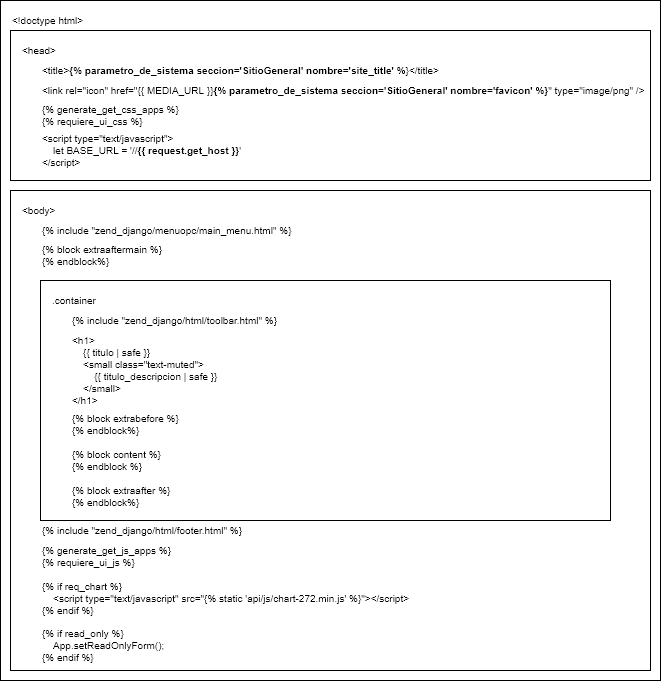
\includegraphics[scale=0.65]{./diagram/html_struct_html}
	\caption{html\_struct.html}
\end{figure}

\section{toolbar.html}

\begin{lstlisting}[language=Python]
toolbar = [
{'type': 'rlink',       'label': 'Etiqueta',    'url': 'http://...'},
{'type': 'link',        'label': 'Etiqueta',    'view': 'NombreVista'},
{'type': 'link_pk',     'label': 'Etiqueta',    'view': 'NombreVista',  pk: 'Valor'},
{'type': 'link_pk_del', 'label': 'Etiqueta',    'view': 'NombreVista',  pk: 'Valor'},
{'type': 'button',      'label': 'Etiqueta',    'onclick': 'CodigoJS'},
{'type': 'search'},
]
\end{lstlisting}

\section{form.html}

\begin{tabular}{|l|l|}
	\hline
	Llamada como & zend\_django/html/form.html \\
	\hline
	Extiende & zend\_django/html/html\_struct.html \\
	\hline
	Carga & crispy\_forms\_tags \\
	& op\_helpers \\
	\hline
\end{tabular}

\begin{lstlisting}
forms = {
	'top': [{'title':'XXXX', 'form': form_object}, ...],
	'left': [...],
	'right': [...],
	'bottom': [...],
}
\end{lstlisting}

\begin{figure}
	\centering
	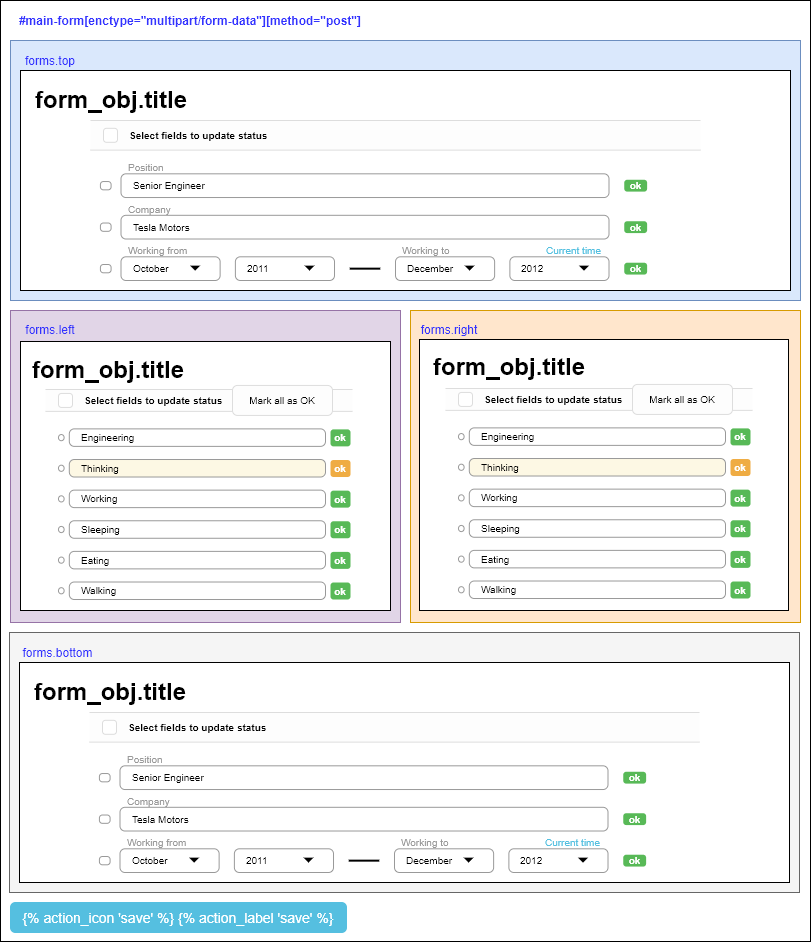
\includegraphics[scale=0.65]{./diagram/forms_html}
	\caption{forms.html}
\end{figure}

\chapter{Utilerías JS}

\section{zend\_django.js}

\subsection{Date}

\begin{description}
	\item[String asMySQL()] Devuelve la fecha en formato MySQL YYYY-MM-DD
	\item[String asMx()] Devuelve la fecha en formato europeo DD-MM-YYYY
	\item[String theTime()] Devuelve la hora en formato hh:mm
	\item[Date fromMX(String date)] Recibe una cadena en formato DD-MM-YYYY y devuelve el objeto tipo Date correspondiente
	\item[Date addDays(int dias)] Suma un numero de días a la fecha
\end{description}

\subsection{Number}

\begin{description}
	\item[String asMoney()] Devuelve el número como cadena en formato de moneda (con dos decimales)
\end{description}

\subsection{clsApp : App}

\begin{description}
	\item[void checkInputIn(String idcontainer)] Activa todas las casillas de verificación contenidas en el contenedor con id = idcontainer
	\item[void uncheckInputIn(String idcontainer)] Desactiva todas las casillas de verificación contenidas en el contenedor con id = idcontainer
	\item[void openPanel(String body, String title, boolean close=true, String footer=null,]
	\item[\quad String idmodal=``modal-panel-message'')] Genera un nuevo panel bootstrap con el contenido de body y el identificador indicado en idmodal
	\item[void closePanel(String idmodal=``modal-panel-message'')] Cierra el panel bootstrap identificado por idmodal
	\item[void setUIControls] Genera los controles UI para navegadores que no soportan controles HTML5 para controles input tipo date
	\item[void setReadOnlyForm(String container\_selector=``\#main-form'')] Aplica readonly a los controles de formulario contenidos en el contenedor indicado por container\_selector
	\item [void showPrivacyPolicy()] Abre en un panel bootstrap el contenido de politica de privacidad, establecido en el elemento HTML con el selector \textit{\#privacy-policy-template}
	\item[void showDeletingConfirmation(String url, String elemento=``elemento'', String pre\_elemento=``el'')] Muestra el panel bootstrap de confirmación de eliminación de `el` `elemento`, el boton de \textit{Aceptar} es un hipervínculo a url
	\item[boolean isEmpty(variant valor)] Indica si es una cadena vacia o vale 0 (cero)
	\item[boolean validate\_required\_fields(String container)] Verifica si todos los controloes dentro del container (selector) tienen un valor establecido
\end{description}

\backmatter
% bibliography, glossary and index would go here.

\end{document}